\section{Технический проект}

\subsection{Архитектура программной системы}

Разрабатываемая система представляет собой программно-информационную систему для организации и проведения занятий йогой — мобильное приложение «Йога-студия» для платформы Android. Приложение построено по принципу Single Activity с использованием фрагментов (Fragments). Архитектурная схема приложения представлена на рисунке \ref{fig:architecture}.

\begin{figure}[H]
	\centering
	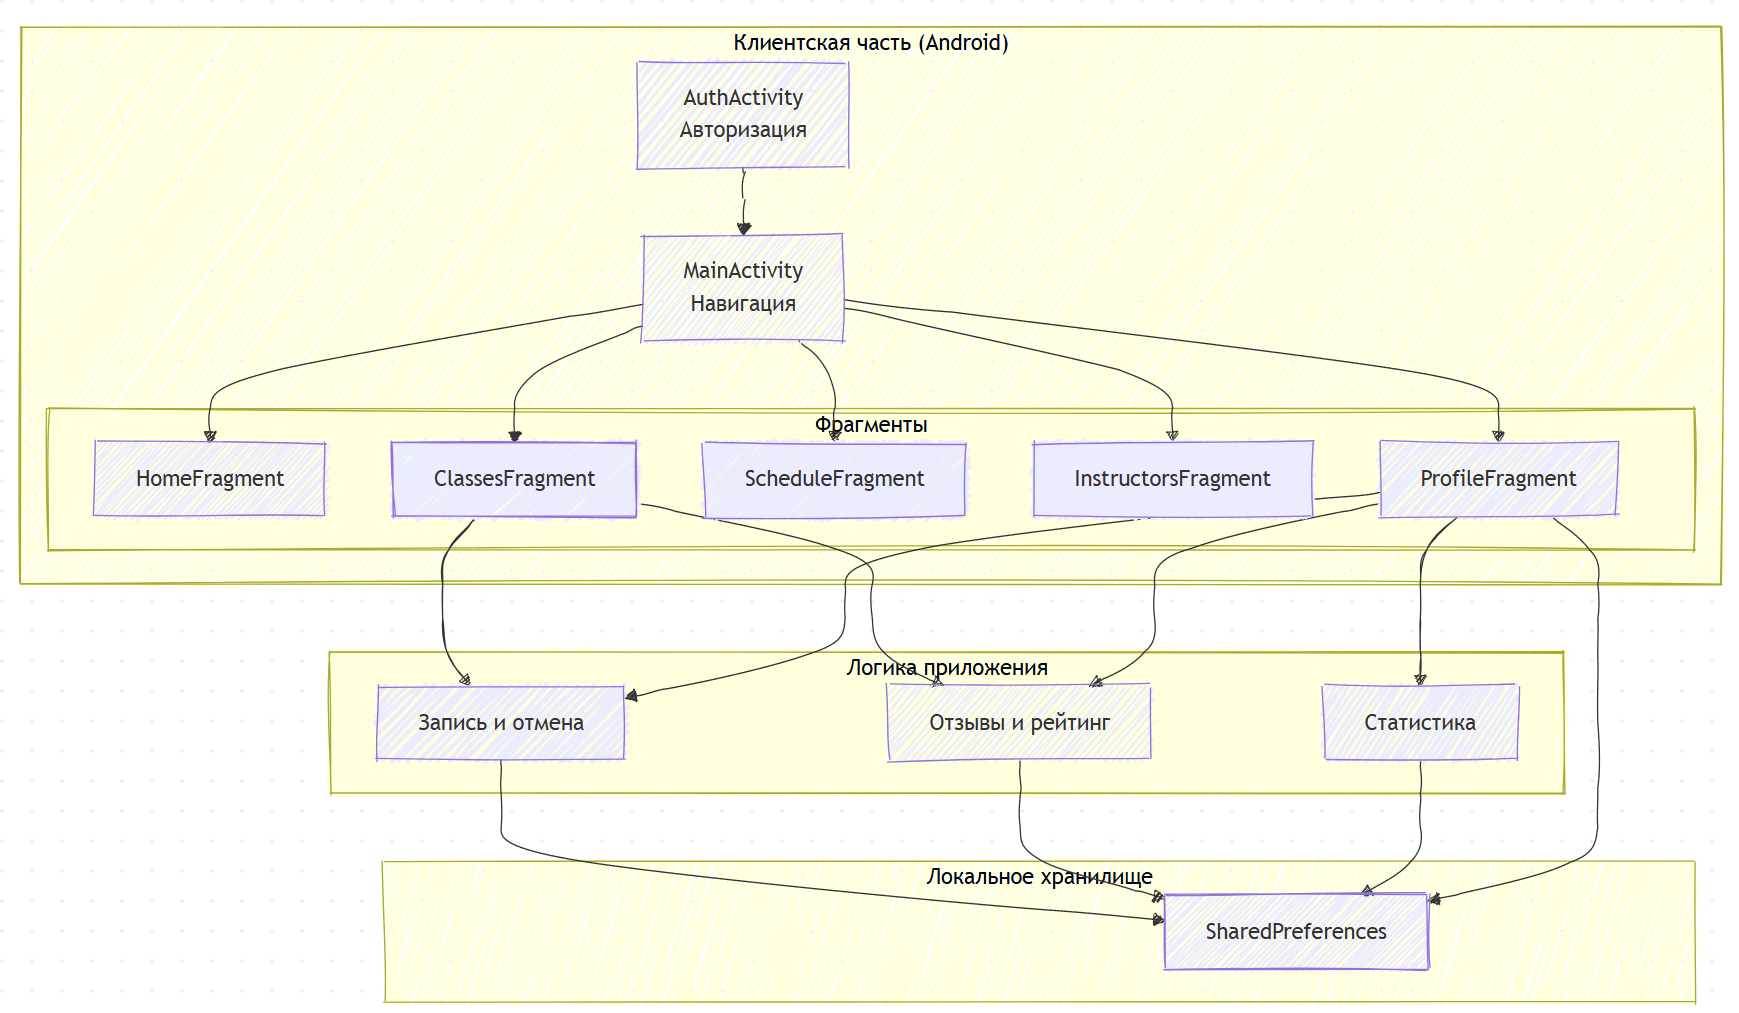
\includegraphics[width=0.9\textwidth]{images/architecture.png}
	\caption{Архитектурная схема приложения «Йога-студия»}
	\label{fig:architecture}
\end{figure}

Выбор такой архитектуры обоснован требованиями проекта: необходимо обеспечить одновременную работу пользовательской части (просмотр занятий, расписания, инструкторов) с единым хранилищем данных. Приложение централизует бизнес-логику и валидацию данных.

\subsection{Обоснование выбора технологий проектирования}

На сегодняшний день рынок мобильных разработок предлагает множество инструментов для создания приложений. Для достижения поставленной цели были выбраны следующие технологии.

\subsubsection{Kotlin как язык программирования}

Kotlin представляет собой современный статически типизированный язык программирования, работающий поверх Java Virtual Machine (JVM). Данный язык был официально рекомендован компанией Google для разработки под Android в 2017 году. Основными преимуществами Kotlin являются лаконичный и выразительный синтаксис, полная совместимость с Java, позволяющая использовать существующие Java-библиотеки, а также null-безопасность, которая существенно снижает количество ошибок во время выполнения. Кроме того, Kotlin поддерживает корутины для асинхронного программирования и имеет официальную поддержку в среде разработки Android Studio.

\subsubsection{Android SDK как фреймворк разработки}

Android Software Development Kit (SDK) представляет собой набор инструментов для разработки приложений под Android, включающий библиотеки, отладчик, эмулятор и документацию. В рамках данного проекта используются следующие основные компоненты Android SDK. Activity является основным компонентом для управления экранами. Fragment используется для создания модульных интерфейсов. RecyclerView применяется для отображения списков, таких как списки занятий и инструкторов. ViewPager2 используется для создания вкладок, в частности на экране авторизации.

\subsubsection{SharedPreferences как способ хранения данных}

Для хранения пользовательских данных, включая профиль, записи, отзывы и прогресс, используются SharedPreferences. Данный механизм представляет собой хранение пар «ключ-значение» локально на устройстве. Основными преимуществами SharedPreferences являются отсутствие необходимости подключения к интернету, простота реализации и сохранение данных даже после перезапуска приложения.

SharedPreferences поддерживает следующие типы данных: строки (String), целые числа (Int), логические значения (Boolean), числа с плавающей точкой (Float, Long), а также наборы строк (Set<String>). Для хранения сложных структур данных (например, списка занятий) используется преобразование в JSON-строку с помощью библиотеки Gson.

\subsubsection{Интеграция с MPAndroidChart для построения графиков}

Для визуализации прогресса пользователя в виде графиков используется библиотека MPAndroidChart. Данная библиотека предоставляет широкие возможности для построения различных типов диаграмм, включая линейные графики, гистограммы и круговые диаграммы. Библиотека имеет открытый исходный код и активно поддерживается сообществом разработчиков.

\subsection{Клиентская часть}

\subsubsection{Структура Activity и Fragments}

Приложение построено по принципу Single Activity с использованием фрагментов (Fragments). Основными компонентами приложения являются AuthActivity, представляющий собой экран авторизации и регистрации с вкладками, а также MainActivity, который является основным экраном с навигацией на основе BottomNavigationView.

Фрагмент HomeFragment отвечает за главный экран, отображающий приветствие, статистику и рекомендации. Фрагмент ClassesFragment реализует каталог занятий со списком и фильтрацией по городу. Фрагмент ScheduleFragment обеспечивает отображение расписания с календарём и списком занятий. Фрагмент InstructorsFragment отображает список инструкторов с фильтрацией по городу. Фрагмент ProfileFragment предоставляет профиль пользователя с аватаром и настройками.

Отдельные Activity используются для списка записей пользователя (MyBookingsActivity), экрана отзыва с рейтингом и комментарием (ReviewActivity), а также экрана статистики и графиков (ProgressActivity).

\subsubsection{Навигация и пользовательский интерфейс}

Навигация между разделами осуществляется с помощью BottomNavigationView, который позволяет переключаться между пятью основными экранами: главным, каталогом занятий, расписанием, инструкторами и профилем. При переходе между вкладками происходит замена одного фрагмента на другой в контейнере, расположенном в MainActivity. Пользовательский интерфейс выполнен с использованием компонентов Material Design, что обеспечивает современный внешний вид и интуитивно понятное взаимодействие.

\subsection{Диаграмма компонентов}

На рисунке \ref{fig:component} представлена диаграмма компонентов приложения, отражающая модульную структуру.

\begin{figure}[H]
	\centering
	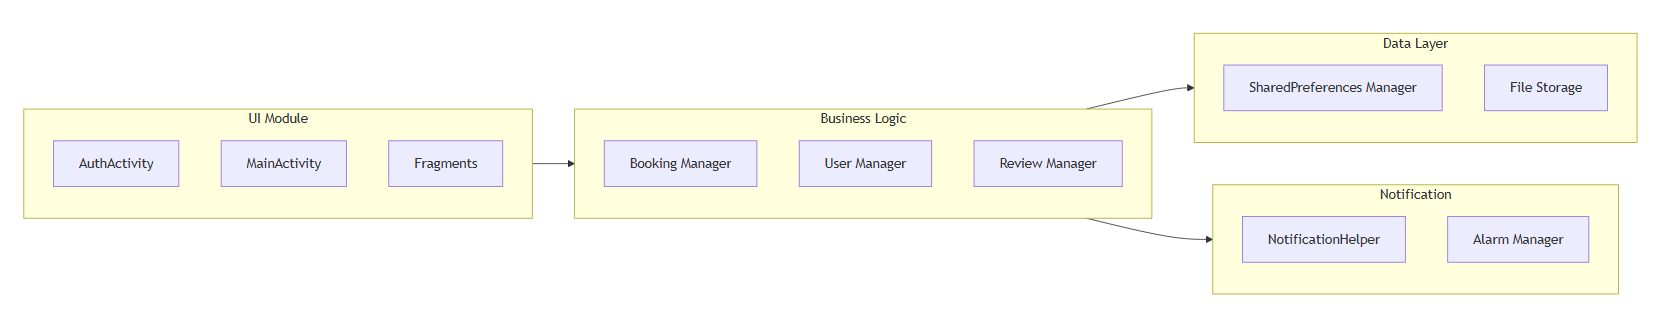
\includegraphics[width=0.9\textwidth]{images/component-diagram.png}
	\caption{Диаграмма компонентов}
	\label{fig:component}
\end{figure}

Приложение включает следующие компоненты: модуль авторизации (отвечает за вход и регистрацию пользователей), модуль навигации (обеспечивает переключение между вкладками), модуль занятий (управляет отображением каталога и деталей занятий), модуль расписания (предоставляет календарь и список занятий), модуль профиля (хранит и редактирует данные пользователя), модуль записей (управляет записью и отменой занятий), модуль отзывов (обрабатывает отзывы и рейтинг занятий), модуль статистики (отображает прогресс в виде графиков), модуль уведомлений (отправляет напоминания о занятиях).

\subsection{Диаграмма классов}

На рисунке \ref{fig:classdiagram} приведена диаграмма классов, отражающая объектную модель предметной области.

\begin{figure}[H]
	\centering
	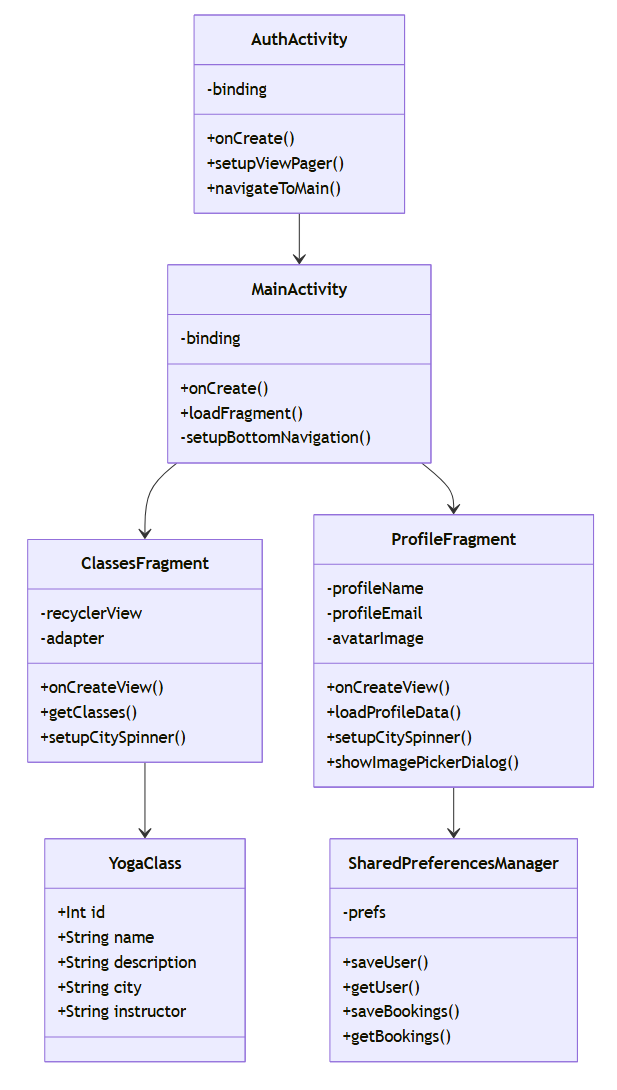
\includegraphics[width=0.7\textwidth]{images/class-diagram.png}
	\caption{Диаграмма классов}
	\label{fig:classdiagram}
\end{figure}

Основными классами приложения являются User (пользователь), Class (занятие), Instructor (инструктор), Booking (запись), Review (отзыв), Progress (прогресс). Класс User связан с Booking и Review. Класс Class связан с Instructor и Booking. Класс Progress связан с User.

\subsection{Диаграмма последовательности}

На рисунке \ref{fig:sequence} показана диаграмма последовательности для сценария «Запись на занятие», демонстрирующая взаимодействие компонентов.

\begin{figure}[H]
	\centering
	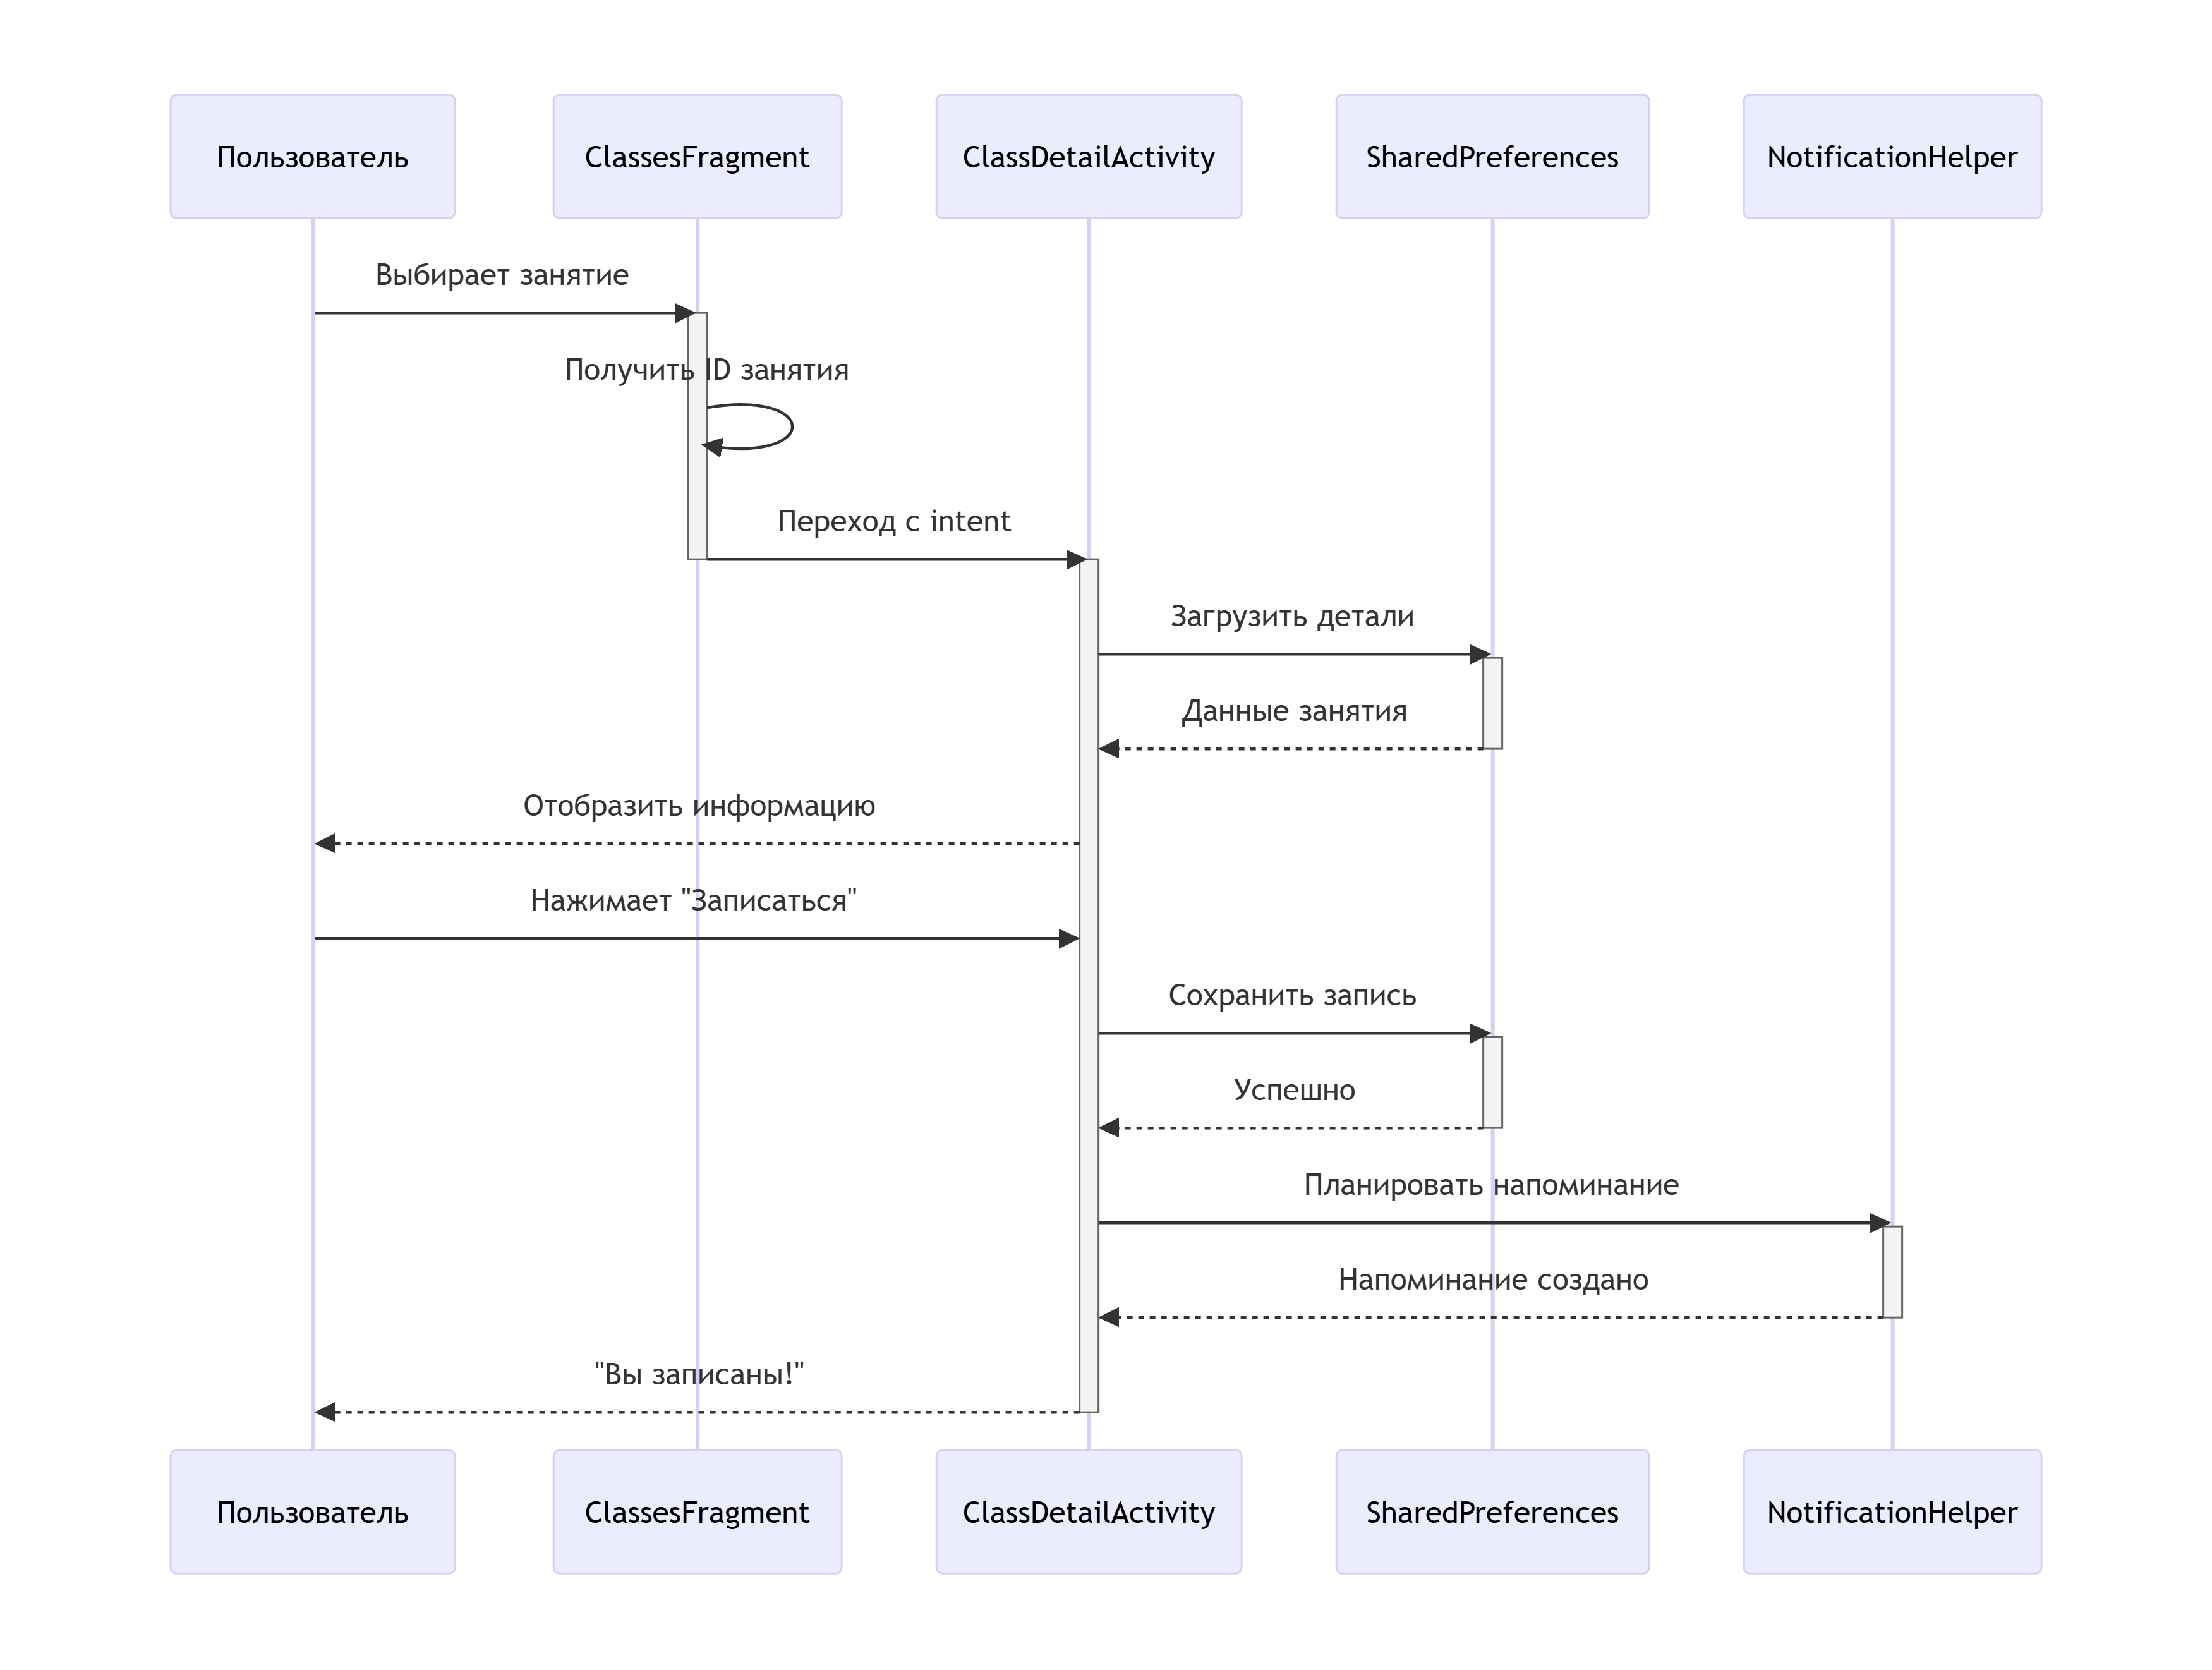
\includegraphics[width=0.9\textwidth]{images/sequence-diagram.png}
	\caption{Диаграмма последовательности (сценарий записи на занятие)}
	\label{fig:sequence}
\end{figure}

Пользователь выбирает занятие в ClassesFragment, система открывает экран деталей. При нажатии кнопки «Записаться» система проверяет наличие свободных мест в SharedPreferences. Если места есть, запись сохраняется, и отправляется уведомление через NotificationHelper.

\subsection{Диаграмма состояний}

На рисунке \ref{fig:state} представлена диаграмма состояний для жизненного цикла записи на занятие.

\begin{figure}[H]
	\centering
	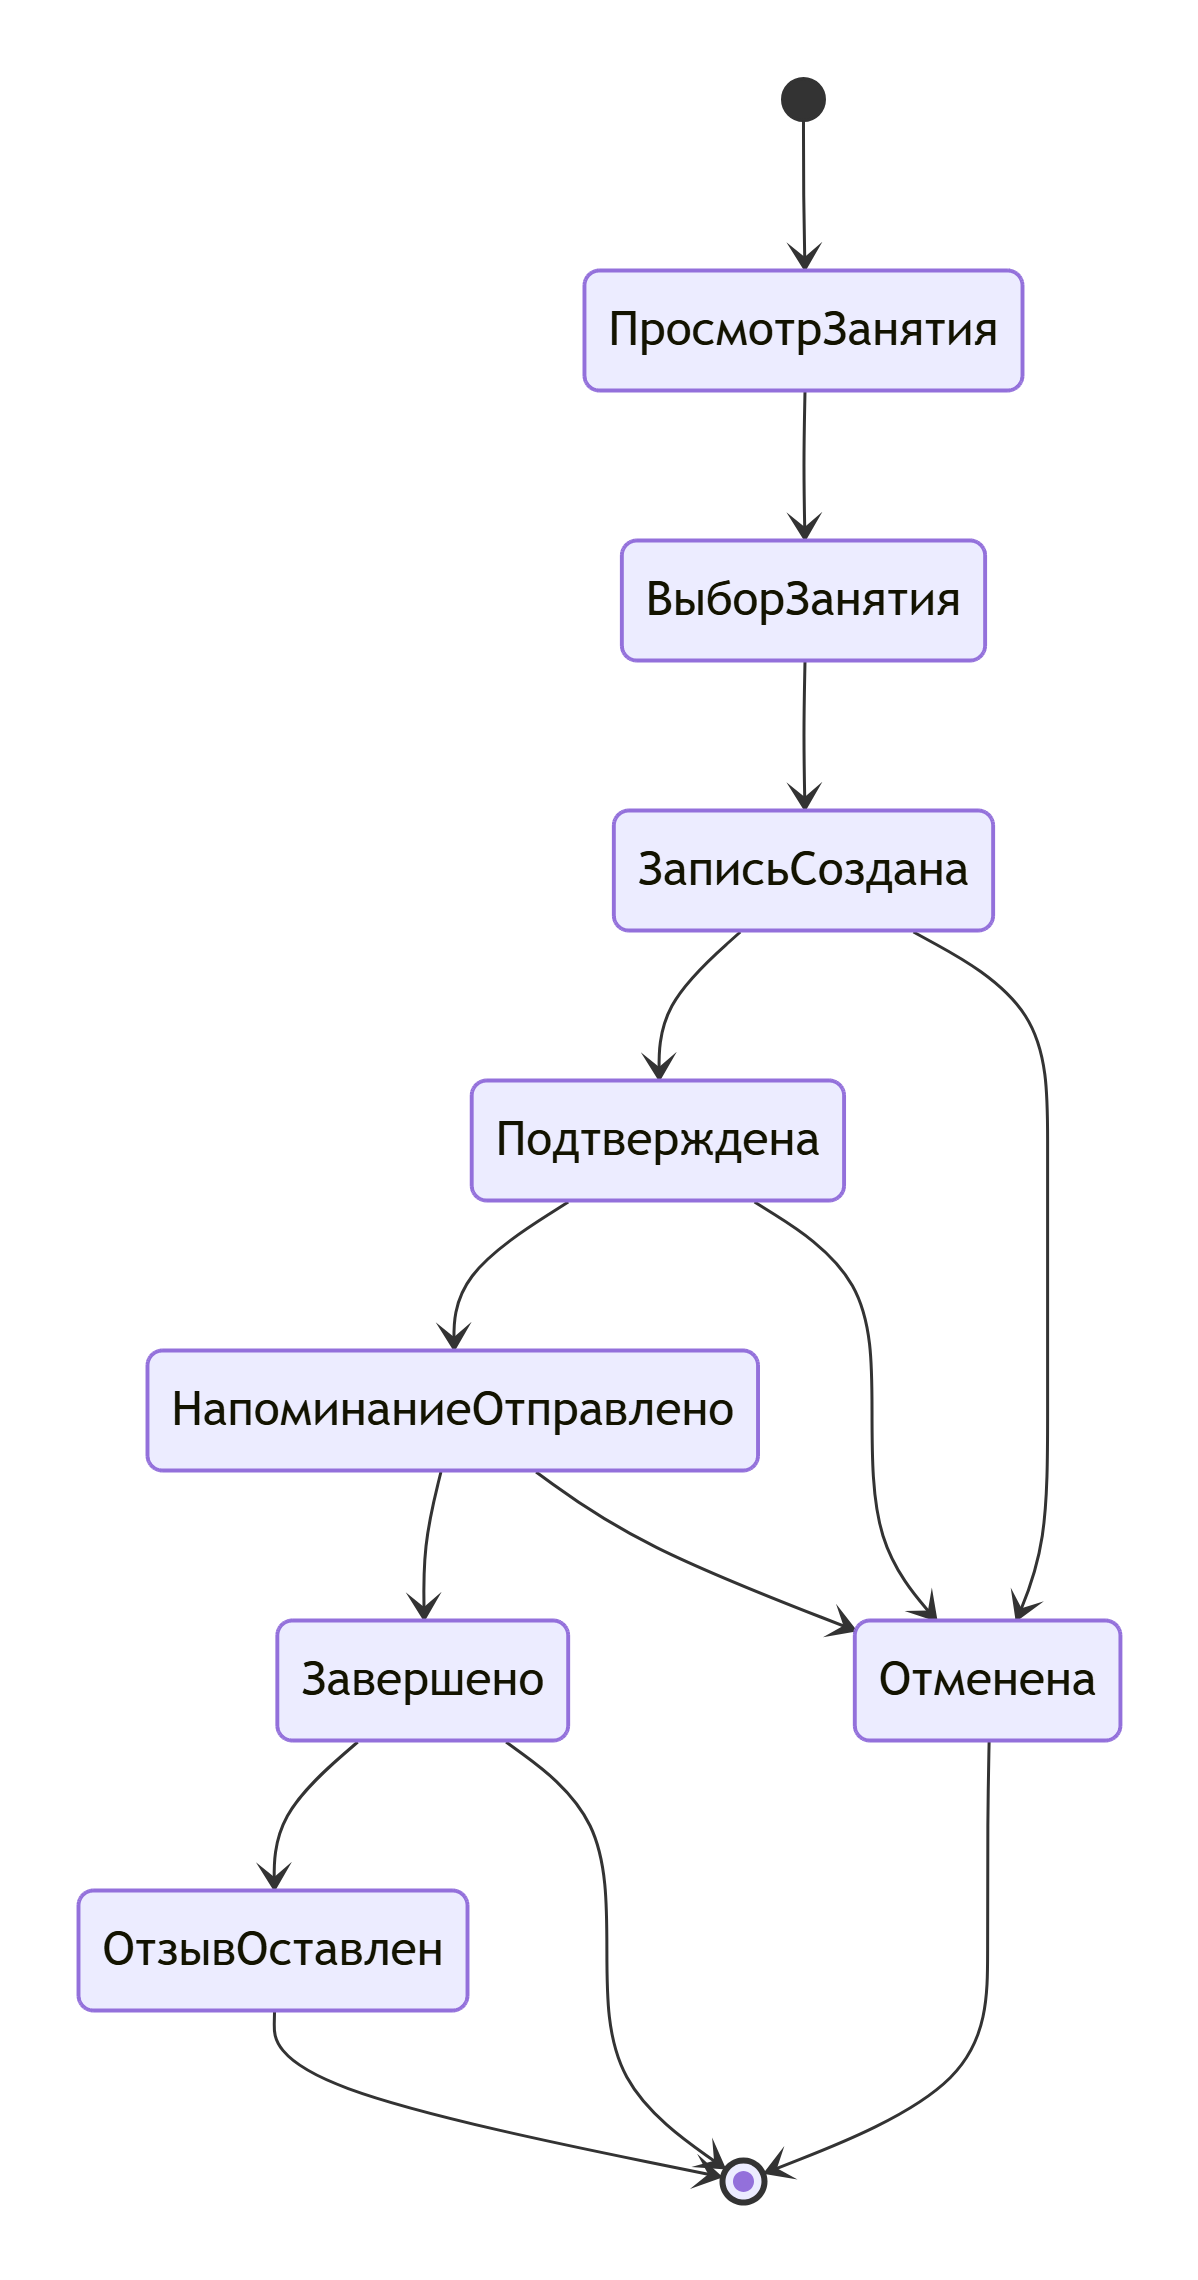
\includegraphics[width=0.7\textwidth]{images/state-diagram.png}
	\caption{Диаграмма состояний записи на занятие}
	\label{fig:state}
\end{figure}

Запись может находиться в следующих состояниях: просмотр занятия, выбор занятия, запись создана, подтверждена, напоминание отправлено, завершено, отменена, отзыв оставлен.

\subsection{Диаграмма взаимодействия фрагментов}

На рисунке \ref{fig:fragment} представлена диаграмма взаимодействия фрагментов в MainActivity, показывающая, как BottomNavigationView управляет загрузкой фрагментов.

\begin{figure}[H]
	\centering
	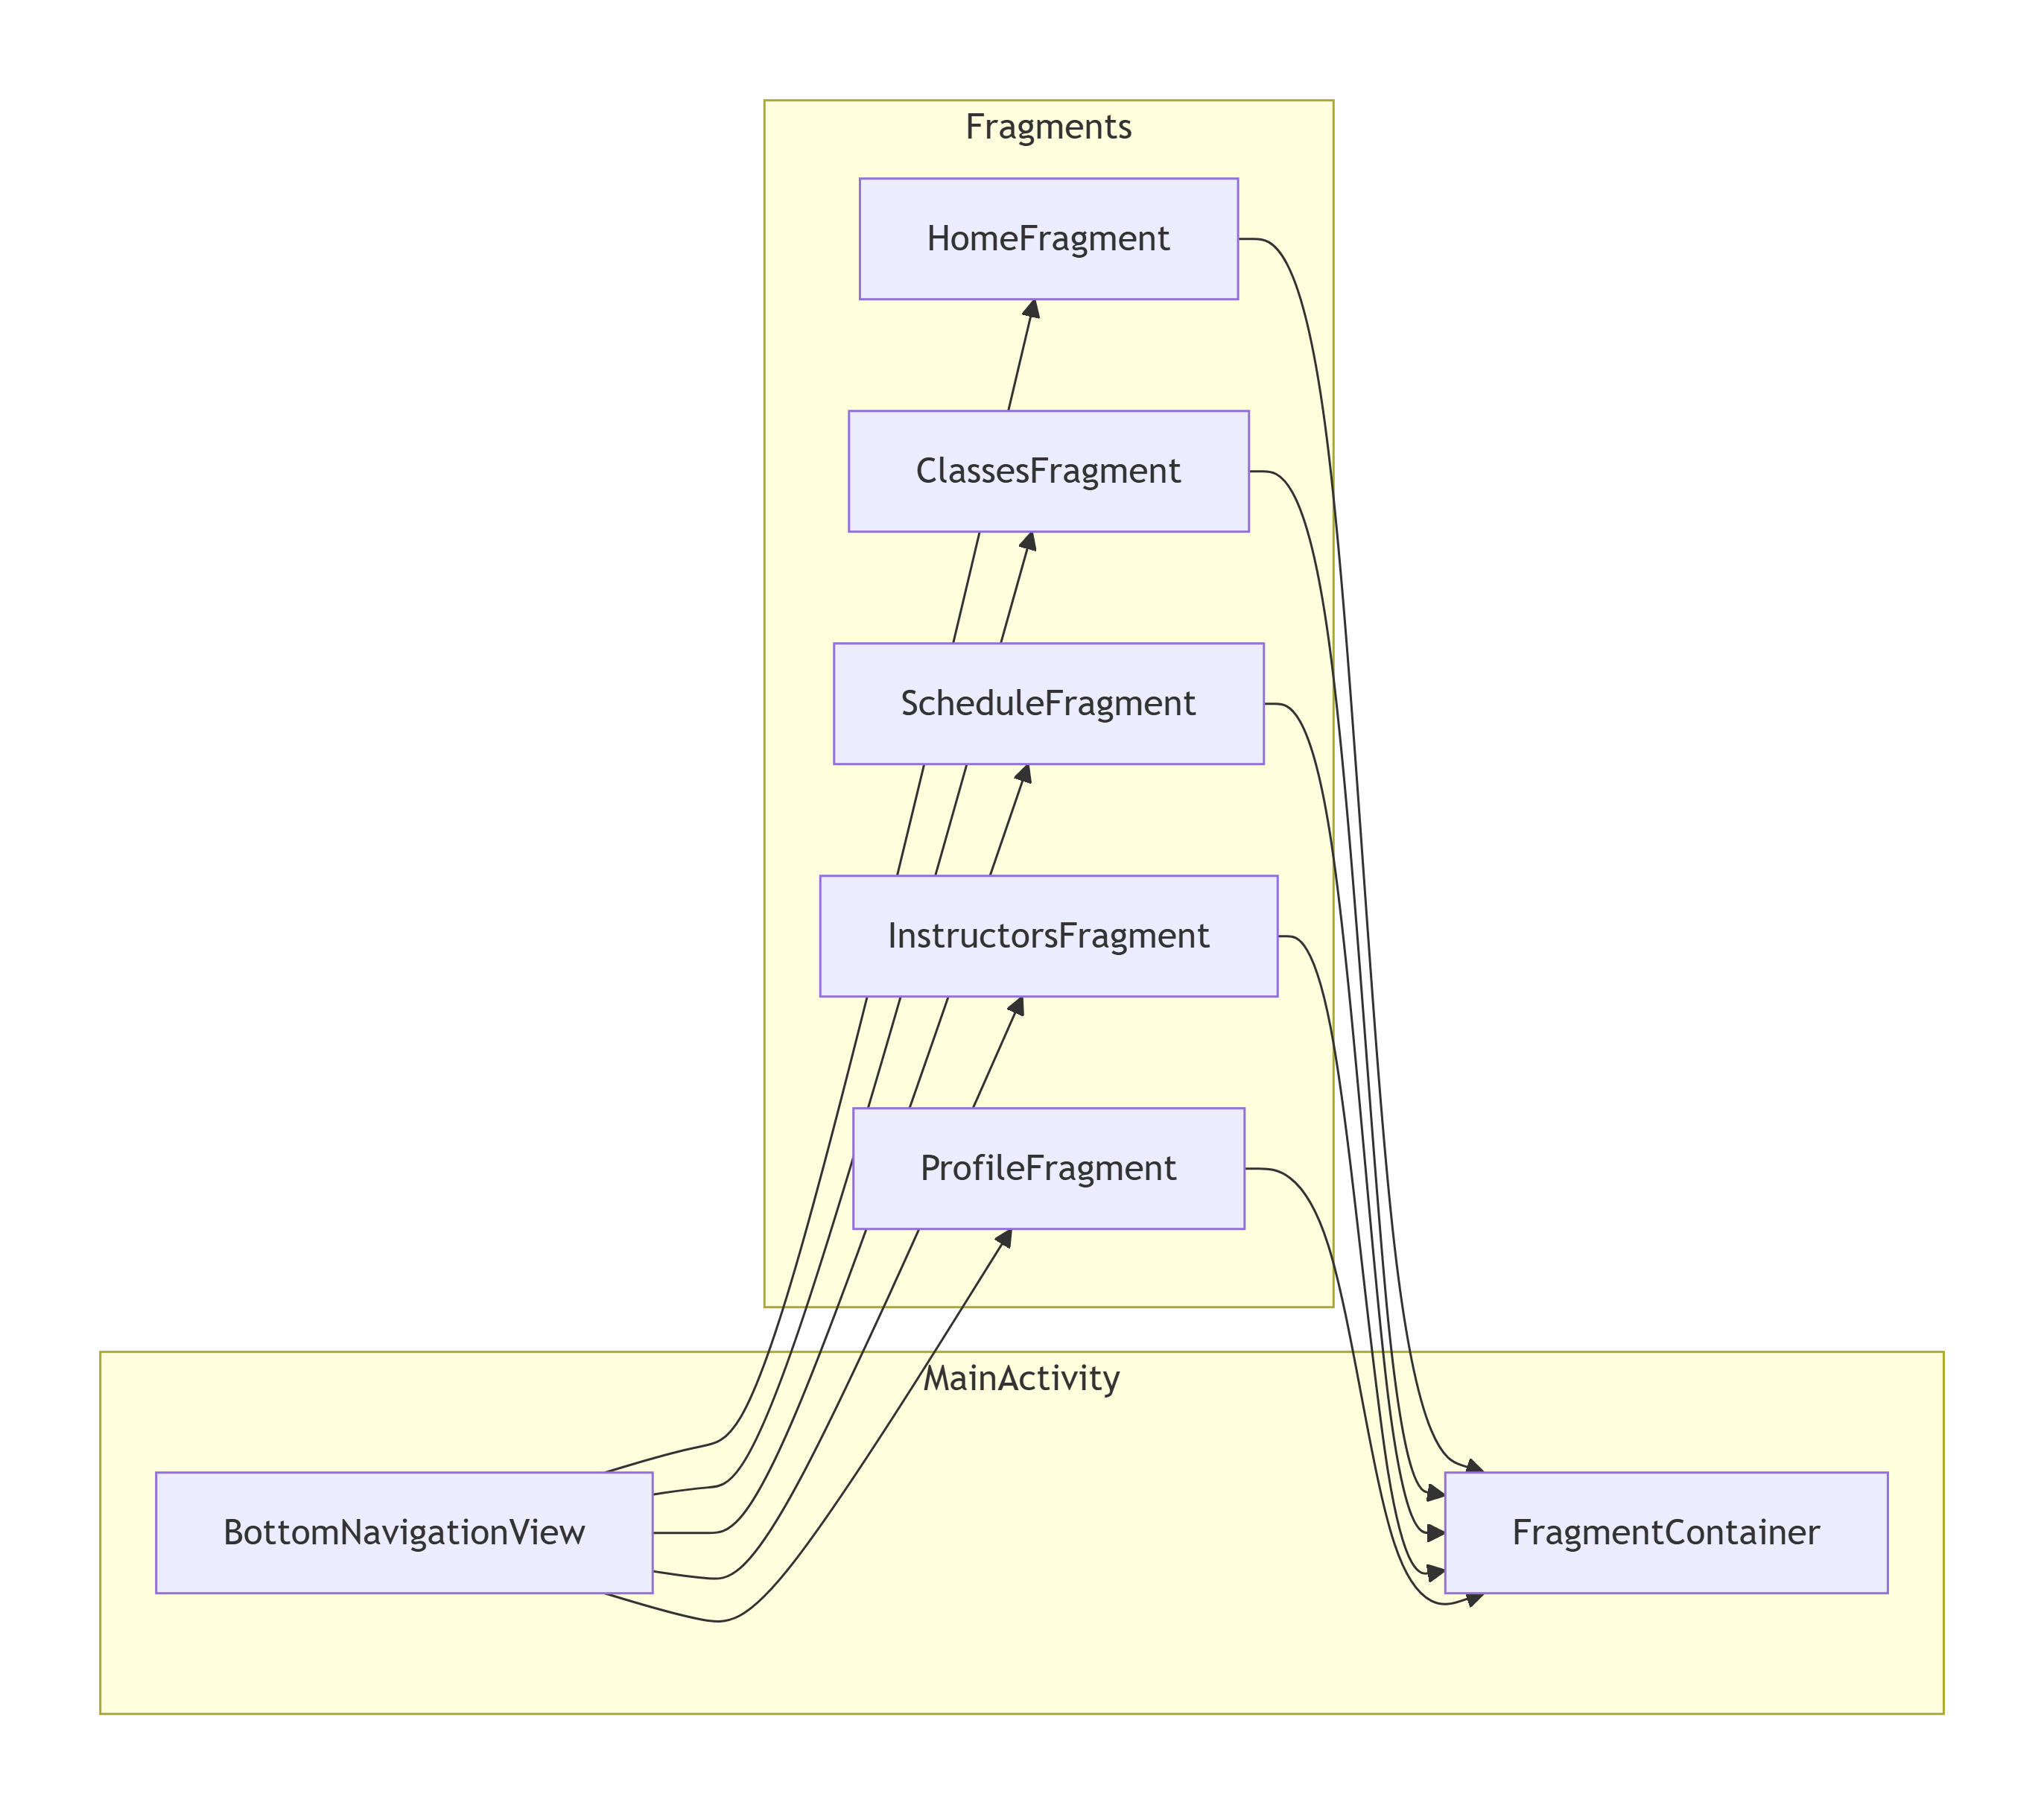
\includegraphics[width=0.9\textwidth]{images/fragment-interaction.png}
	\caption{Диаграмма взаимодействия фрагментов}
	\label{fig:fragment}
\end{figure}

BottomNavigationView обрабатывает выбор пункта меню и заменяет текущий фрагмент на соответствующий выбранному. Для управления фрагментами используется FragmentManager.

\subsection{Диаграмма пакетов}

На рисунке \ref{fig:package} представлена диаграмма пакетов, отражающая модульную структуру приложения на уровне пакетов.

\begin{figure}[H]
	\centering
	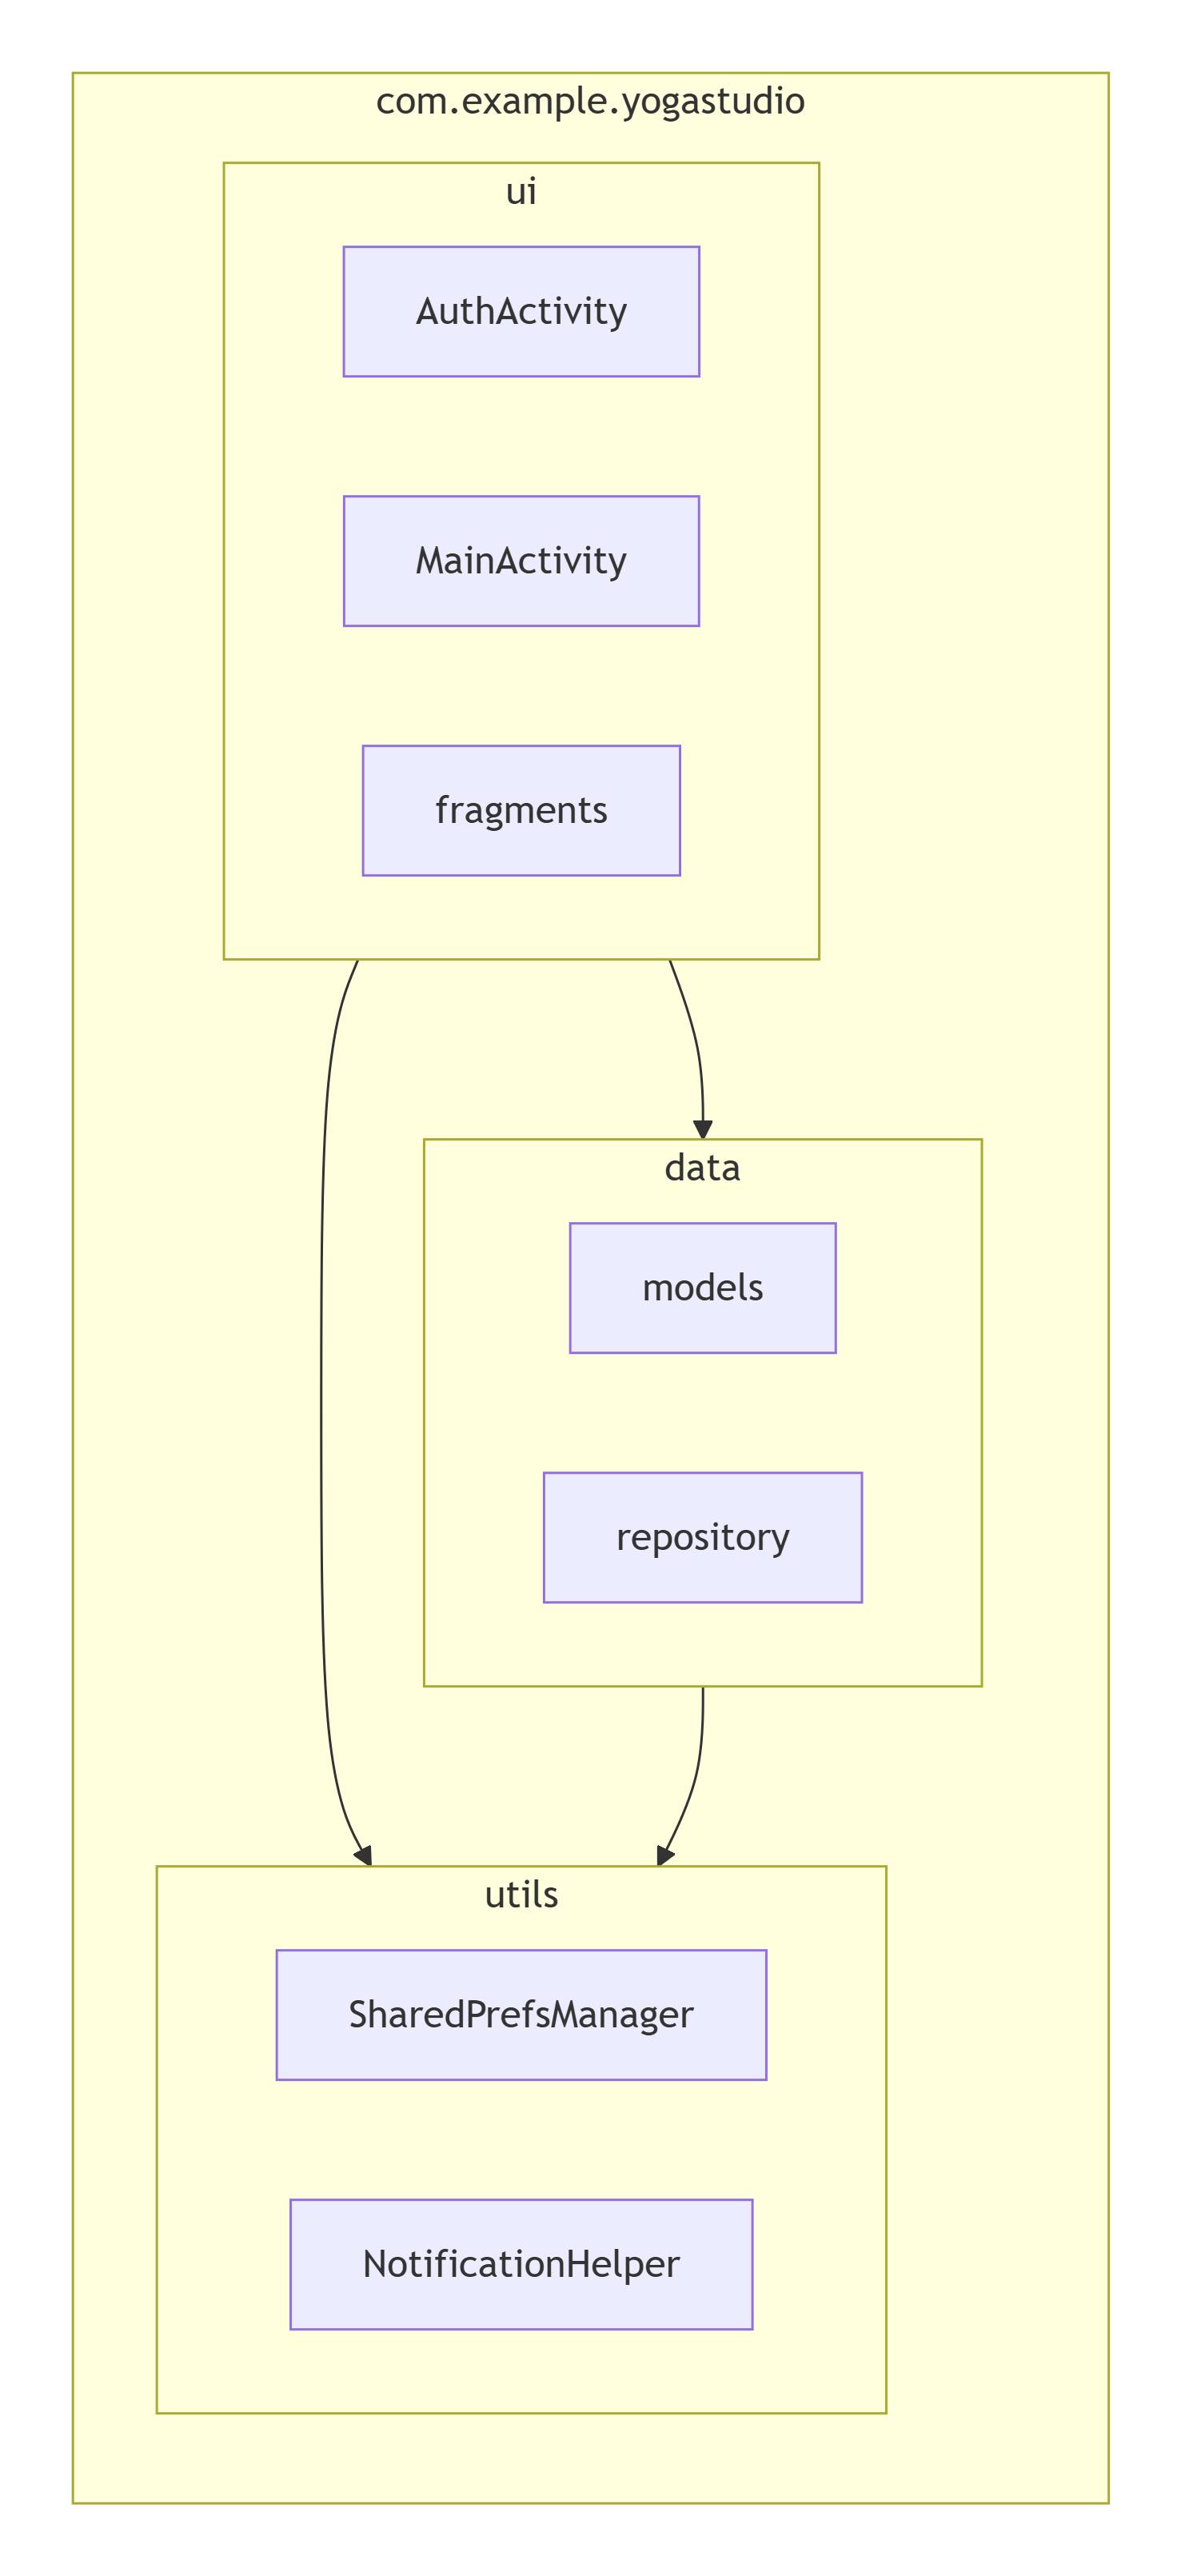
\includegraphics[width=0.7\textwidth]{images/package-diagram.png}
	\caption{Диаграмма пакетов}
	\label{fig:package}
\end{figure}

Приложение разделено на следующие пакеты: ui (пользовательский интерфейс), data (работа с данными), model (модели данных), utils (вспомогательные классы), notifications (уведомления).

\subsection{Диаграмма развертывания}

На рисунке \ref{fig:deployment} представлена диаграмма развертывания, показывающая физическую структуру системы: устройство пользователя, операционную систему Android и локальное хранилище.

\begin{figure}[H]
	\centering
	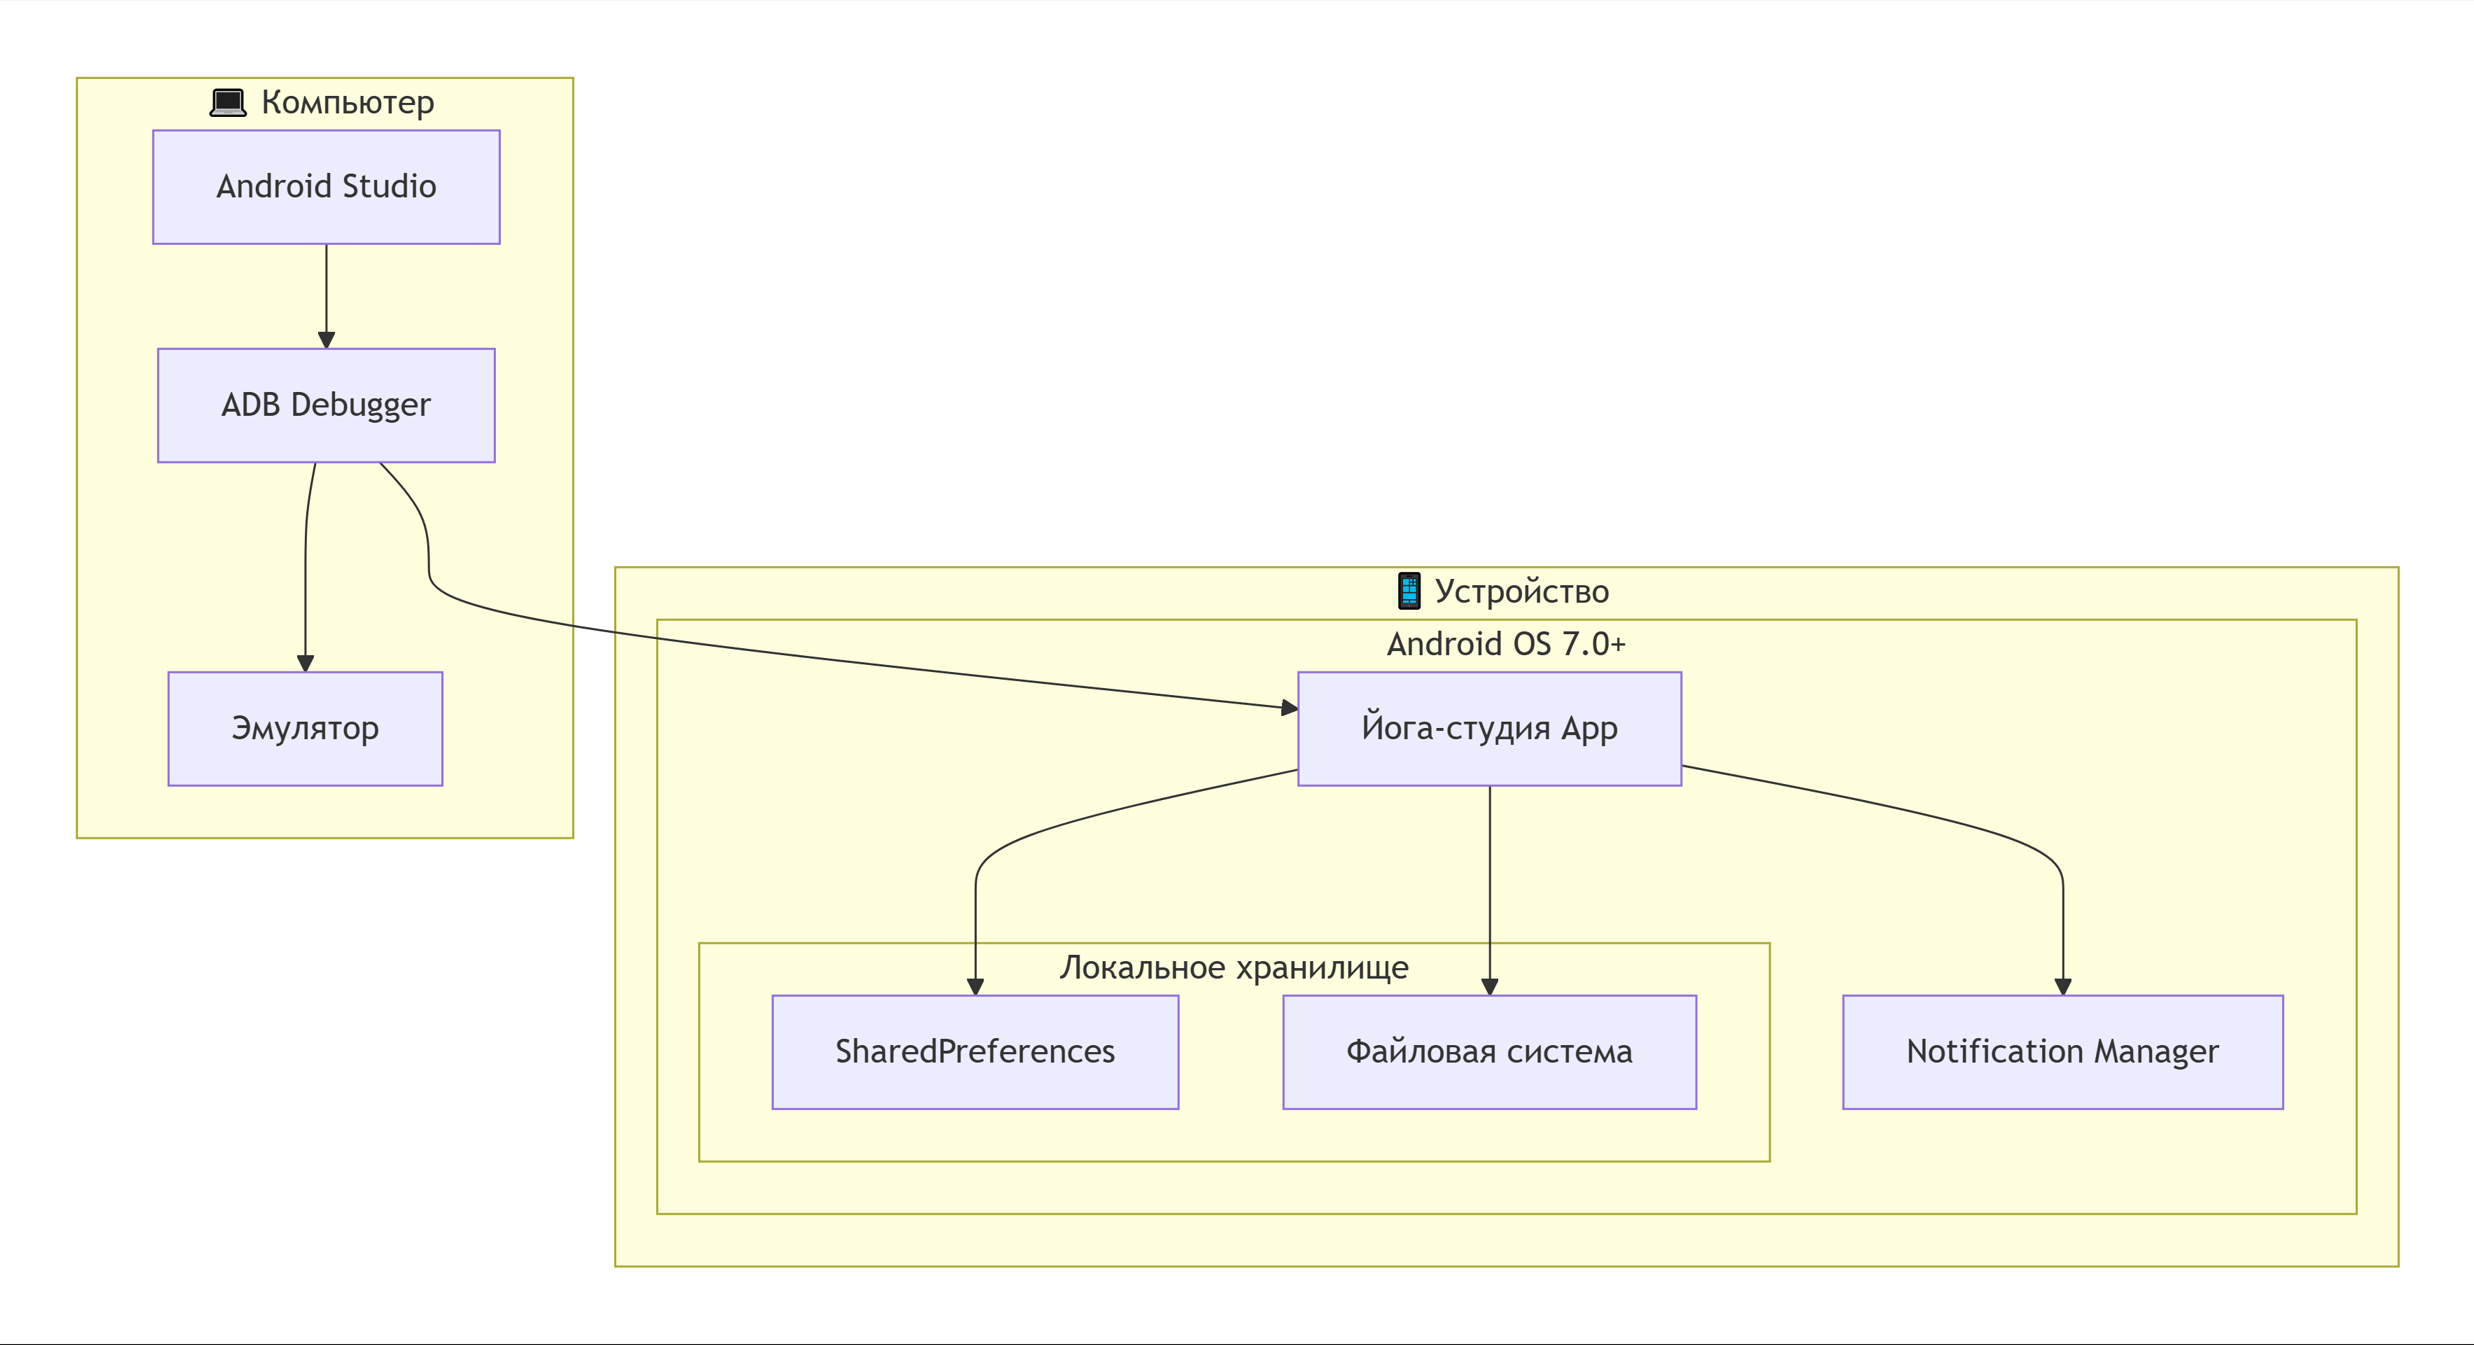
\includegraphics[width=0.9\textwidth]{images/deployment-diagram.png}
	\caption{Диаграмма развертывания}
	\label{fig:deployment}
\end{figure}

Приложение развертывается на физическом устройстве под управлением ОС Android. Для хранения данных используется внутренняя память устройства (SharedPreferences). Для разработки и отладки используется Android Studio с ADB Debugger и эмулятором.

\subsection{Проект базы данных (SharedPreferences)}

\subsubsection{Компоненты хранения данных}

Для хранения данных пользователя используются SharedPreferences, представляющие собой механизм хранения пар «ключ-значение» локально на устройстве. Данные сохраняются в XML-файле в защищённой области приложения. SharedPreferences поддерживает следующие типы данных: строки, целые числа, логические значения, числа с плавающей точкой и наборы строк (StringSet).

\subsubsection{ER-модель данных}

На рисунке \ref{fig:erdiagram} представлена ER-диаграмма сущностей, хранимых в SharedPreferences.

\begin{figure}[H]
	\centering
	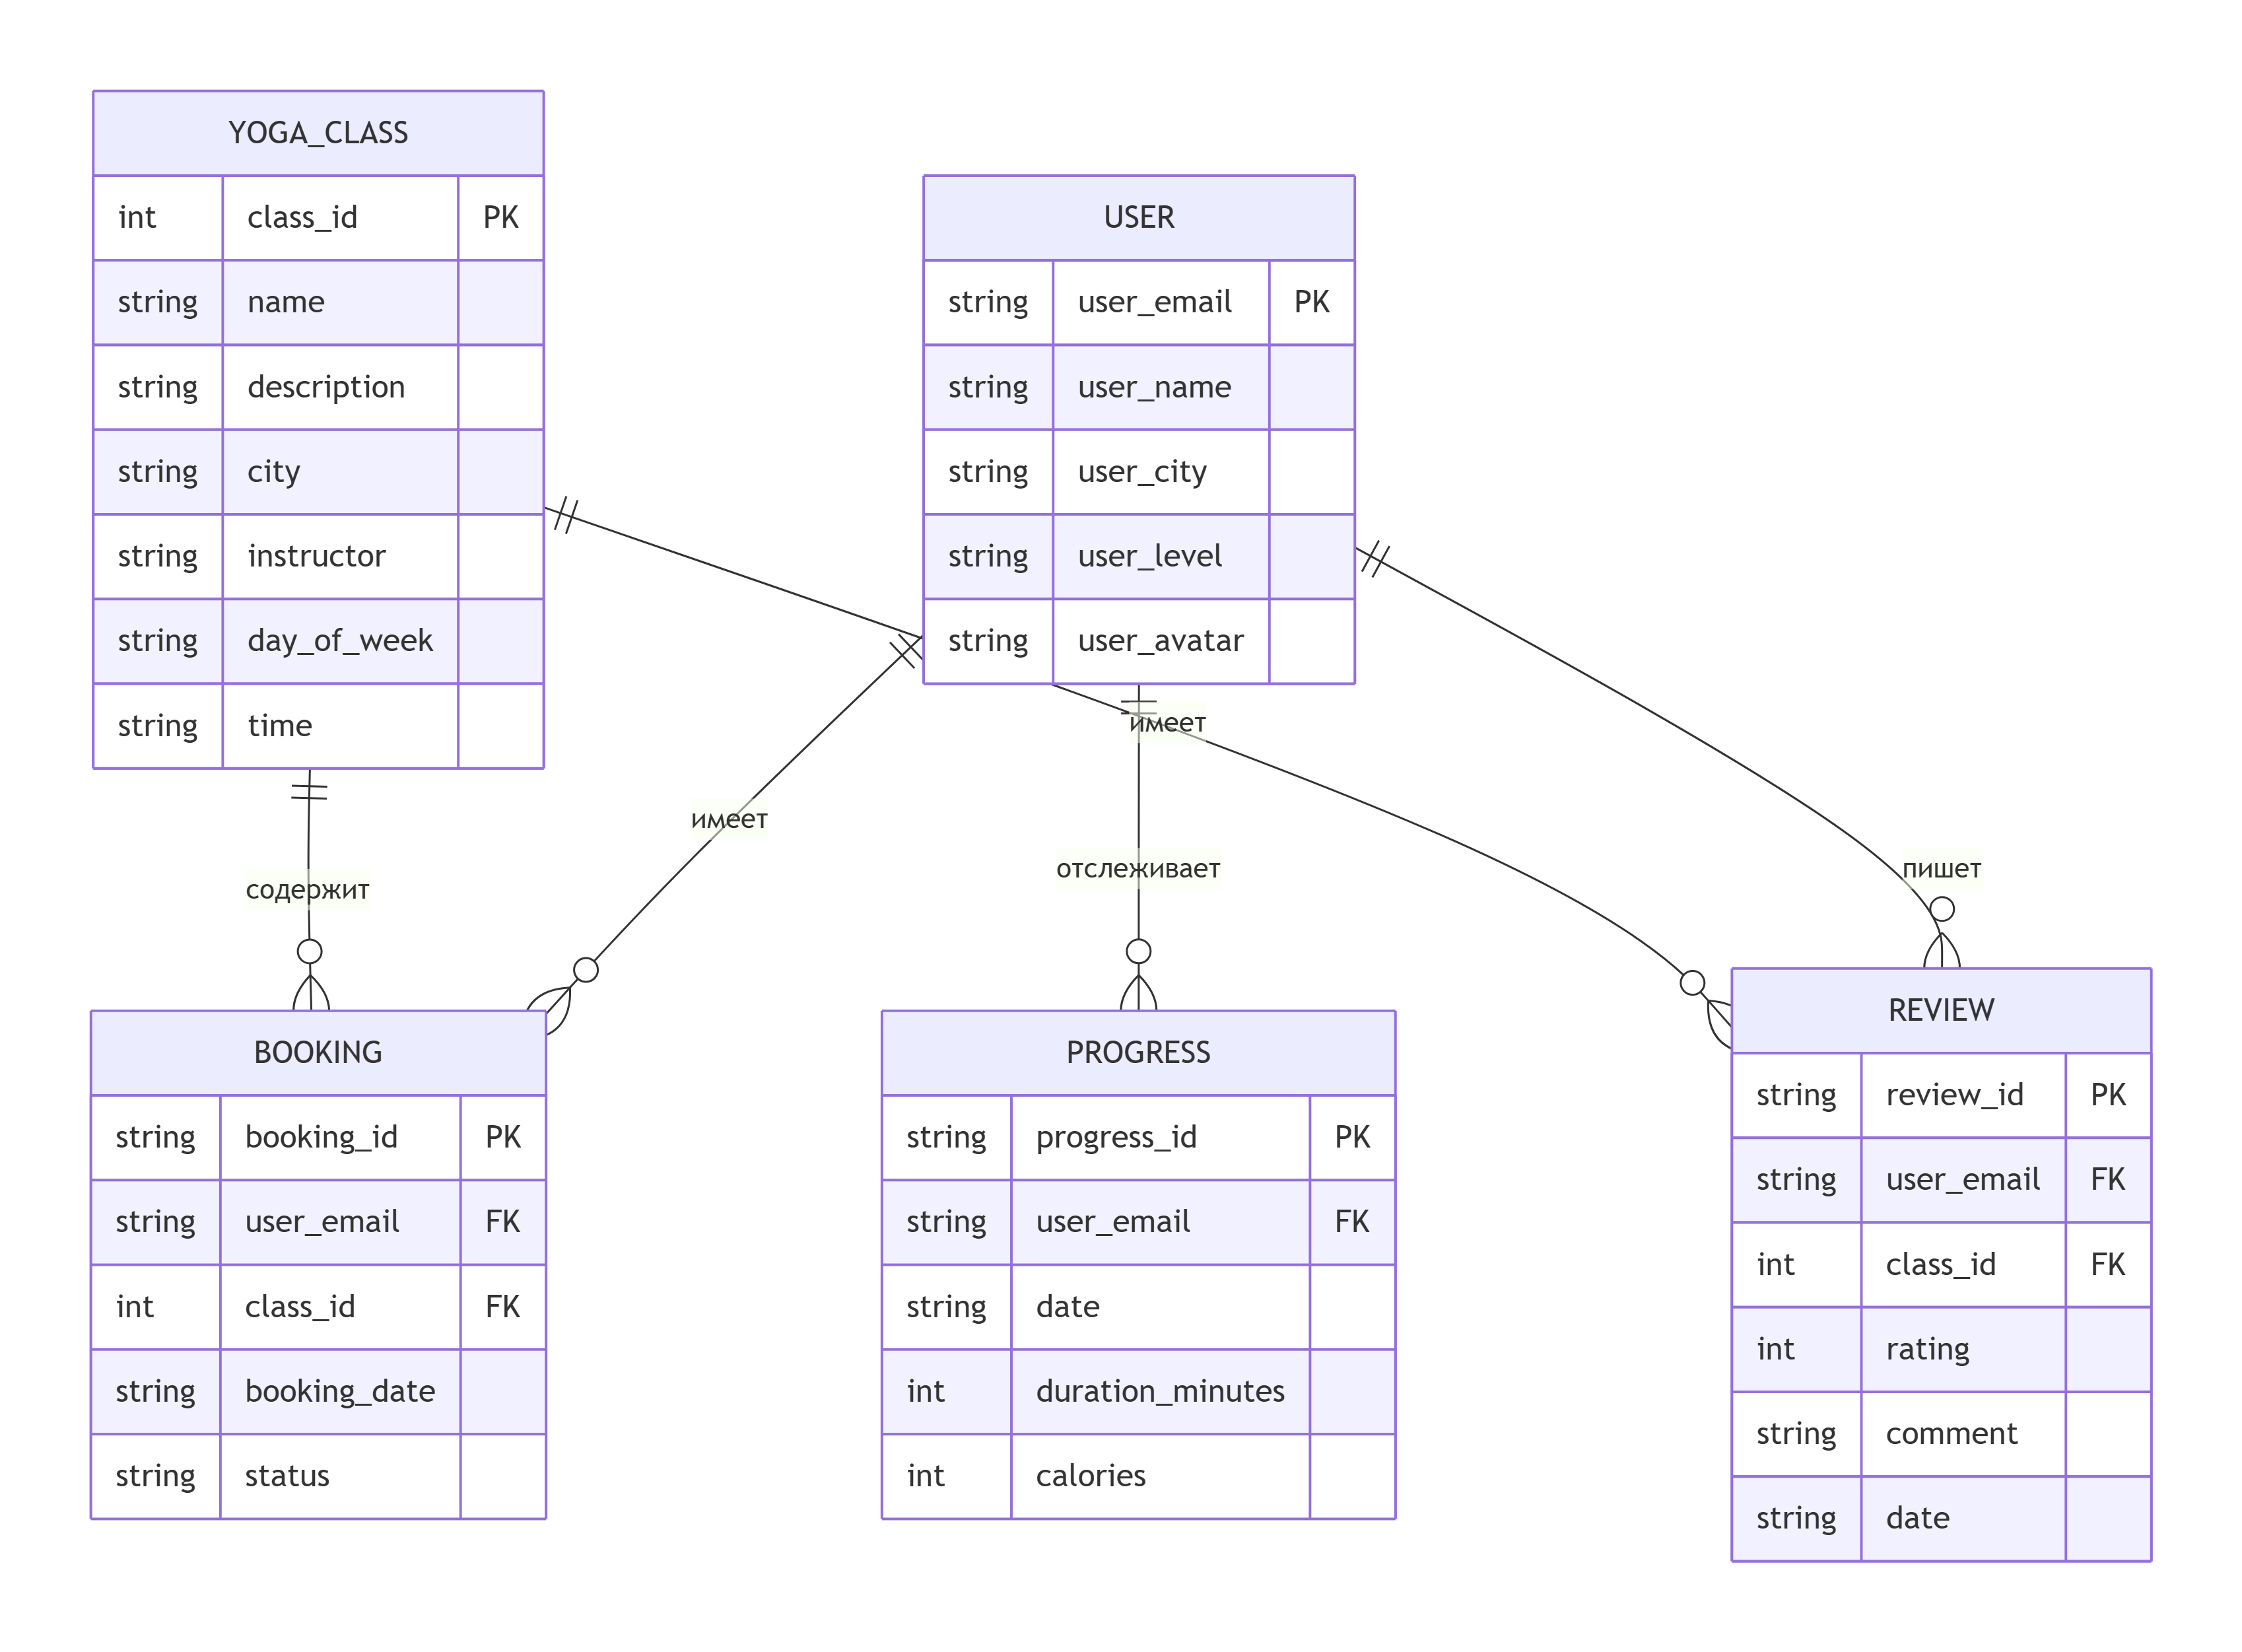
\includegraphics[width=0.9\textwidth]{images/er-diagram.png}
	\caption{ER-диаграмма сущностей}
	\label{fig:erdiagram}
\end{figure}

Ключевыми сущностями являются пользователь (USER), занятие (YOGA\_CLASS), запись (BOOKING), прогресс (PROGRESS) и отзыв (REVIEW). USER связан с BOOKING, PROGRESS и REVIEW. YOGA\_CLASS связан с BOOKING и REVIEW.

\subsubsection{Описание структуры ключей хранилища}

В таблице \ref{tab:sharedprefs} приведено описание основных ключей хранилища SharedPreferences.

\renewcommand{\arraystretch}{1.4}
\begin{table}[H]
	\centering
	\caption{Сущности хранилища SharedPreferences}
	\label{tab:sharedprefs}
	\normalsize
	\setlength{\tabcolsep}{6pt}
	\begin{tabular}{|m{3.3cm}|m{2.2cm}|m{3.5cm}|m{6.5cm}|}
		\hline
		\textbf{Ключ} & \textbf{Тип} & \textbf{Обязательное} & \textbf{Описание} \\
		\hline
		user\_name & String & да & Имя пользователя \\
		\hline
		user\_email & String & да & Адрес электронной почты пользователя \\
		\hline
		user\_avatar & String & нет & URI аватара пользователя \\
		\hline
		user\_city & String & да & Выбранный город (Москва, Санкт-Петербург, Казань) \\
		\hline
		user\_level & String & да & Уровень подготовки \\
		\hline
		user\_styles & StringSet & нет & Любимые стили йоги \\
		\hline
		user\_goals & StringSet & нет & Цели пользователя \\
		\hline
		bookings & StringSet & да & Записи на занятия \\
		\hline
		reviews\_list & String & нет & Список отзывов \\
		\hline
		progress\_list & String & нет & Данные о прогрессе \\
		\hline
		classes\_list & String & да & Список занятий (JSON) \\
		\hline
		instructors\_list & String & да & Список инструкторов (JSON) \\
		\hline
	\end{tabular}
\end{table}
\renewcommand{\arraystretch}{1}

\subsection{Надёжность, производительность и масштабирование}

\subsubsection{Надёжность операций сохранения данных}

Сценарий сохранения данных пользователя реализован с использованием атомарных операций SharedPreferences, что гарантирует целостность данных при любых обстоятельствах. При возникновении ошибки во время сохранения (например, при отсутствии свободного места) система возвращает соответствующее сообщение и не фиксирует частично сохранённые данные.

\subsubsection{Оптимизация загрузки списков}

Для отображения списков занятий, инструкторов и записей используется компонент RecyclerView, который обеспечивает эффективное использование памяти при прокрутке больших объёмов данных. Изображения аватаров пользователей загружаются асинхронно с помощью библиотеки CircleImageView, что предотвращает зависание интерфейса.

\subsubsection{Потенциал масштабирования}

Текущая архитектура допускает дальнейшее масштабирование приложения. При увеличении объёма данных возможен переход от локального хранения SharedPreferences к облачной базе данных (например, Firebase Firestore) без кардинальной перестройки архитектуры. Кроме того, архитектура позволяет добавлять новые типы занятий, категории и фильтры без изменения основных модулей.

\subsection{Информационная безопасность технического проекта}

\subsubsection{Профиль угроз}

Для проекта релевантны следующие угрозы. Несанкционированный доступ к данным пользователя возможен при компрометации устройства. Отправка некорректных или вредоносных данных в SharedPreferences может привести к нарушению целостности информации. Раскрытие внутренних ошибок приложения не должно содержать конфиденциальной информации.

\subsubsection{Меры защиты}

В техническом проекте применяются следующие меры защиты. Пароли пользователей сохраняются в зашифрованном виде с использованием алгоритмов шифрования Android. Все операции с SharedPreferences выполняются в изолированном контейнере приложения. Валидация входных данных выполняется как на уровне пользовательского интерфейса, так и на уровне логики сохранения. Обработка ошибок реализована без вывода стектрейсов и внутренней информации приложения пользователю.

\subsection{Эксплуатация и развёртывание}

\subsubsection{Локальное развёртывание}

Для установки приложения на устройство пользователя необходимо скопировать APK-файл на устройство и разрешить установку из неизвестных источников. Приложение не требует дополнительной настройки после установки. Все данные сохраняются локально и доступны сразу после первого запуска.

\subsubsection{Конфигурация технических средств}

Для работы приложения требуется устройство под управлением операционной системы Android версии не ниже 7.0 (API level 24). Рекомендуемый объём оперативной памяти составляет не менее 2 ГБ. Свободное место на диске для установки приложения должно составлять не менее 50 МБ.

\subsubsection{Требования к устройству}

Минимальные технические требования к устройству включают процессор с частотой не менее 1,2 ГГц, 2 ГБ оперативной памяти и 50 МБ свободного дискового пространства. Устройство должно поддерживать работу с сенсорным экраном и иметь разрешение экрана не менее 480x800 пикселей.

\subsection{Верификация технического проекта}

\subsubsection{Функциональная верификация}

Функциональная верификация должна покрывать следующие сценарии. Проверка авторизации и регистрации пользователей с корректными и некорректными данными. Проверка фильтрации занятий по городу. Проверка записи на занятие и отмены записи. Проверка редактирования профиля пользователя. Проверка отображения графиков прогресса. Проверка оставления отзывов и рейтинга. Проверка получения уведомлений и напоминаний.

\subsubsection{Техническая верификация}

Техническая верификация должна включать проверку целостности данных после операций сохранения, проверку корректности работы приложения при отсутствии свободного места на устройстве, проверку работы приложения при сворачивании и восстановлении, а также проверку производительности при увеличении объёма данных.

\subsection{Выводы по разделу}

В данном разделе представлены архитектура и компоненты разрабатываемого мобильного приложения. Обоснован выбор технологий, включая язык Kotlin, Android SDK и SharedPreferences. Разработаны и представлены диаграммы, выполненные на языке UML: архитектурная схема, диаграмма компонентов, диаграмма классов, диаграмма последовательности, диаграмма деятельности, диаграмма состояний, диаграмма взаимодействия фрагментов, диаграмма пакетов, диаграмма развертывания, а также ER-диаграмма. Описаны основные сущности, хранимые в SharedPreferences. Разработанная архитектура обеспечивает модульность, удобство поддержки и масштабирования приложения.